\section{Erstellung des Farbschemas}
\label{sec:farbschema}

In diesem Abschnitt wird eine Methode zur Lösung des Teilproblems $f_{scheme}: FGs \to P$ vorgeschlagen. Hierbei werden Farben aus $P$ für die Funktionsgruppen eines Layouts festgelegt, wodurch die Farbgestaltung der Webseite definiert wird. Zur Veranschaulichung wird ein prototypisches Layout für Musikstreaming verwendet. Es enthält die in \autoref{sec:architektur} festgelegten Funktionsgruppen $FGs = $ \{Primär, Sekundär, Akzent, Interaktion, Text (neutral), Hintergrund (neutral)\}. \autoref{fig:fgs} hebt die Funktionsgruppen des Layouts separat hervor. Für die Funktionsgruppen \{Primär, Sekundär, Akzent, Interaktion\} werden Farben verwendet, die aus ACoPa resultieren. Für die Funktionsgruppen \{Text (neutral), Hintergrund (neutral)\} wird der Suchraum auf $weiss$ und $schwarz$ beschränkt.

\begin{figure}[]
\centering
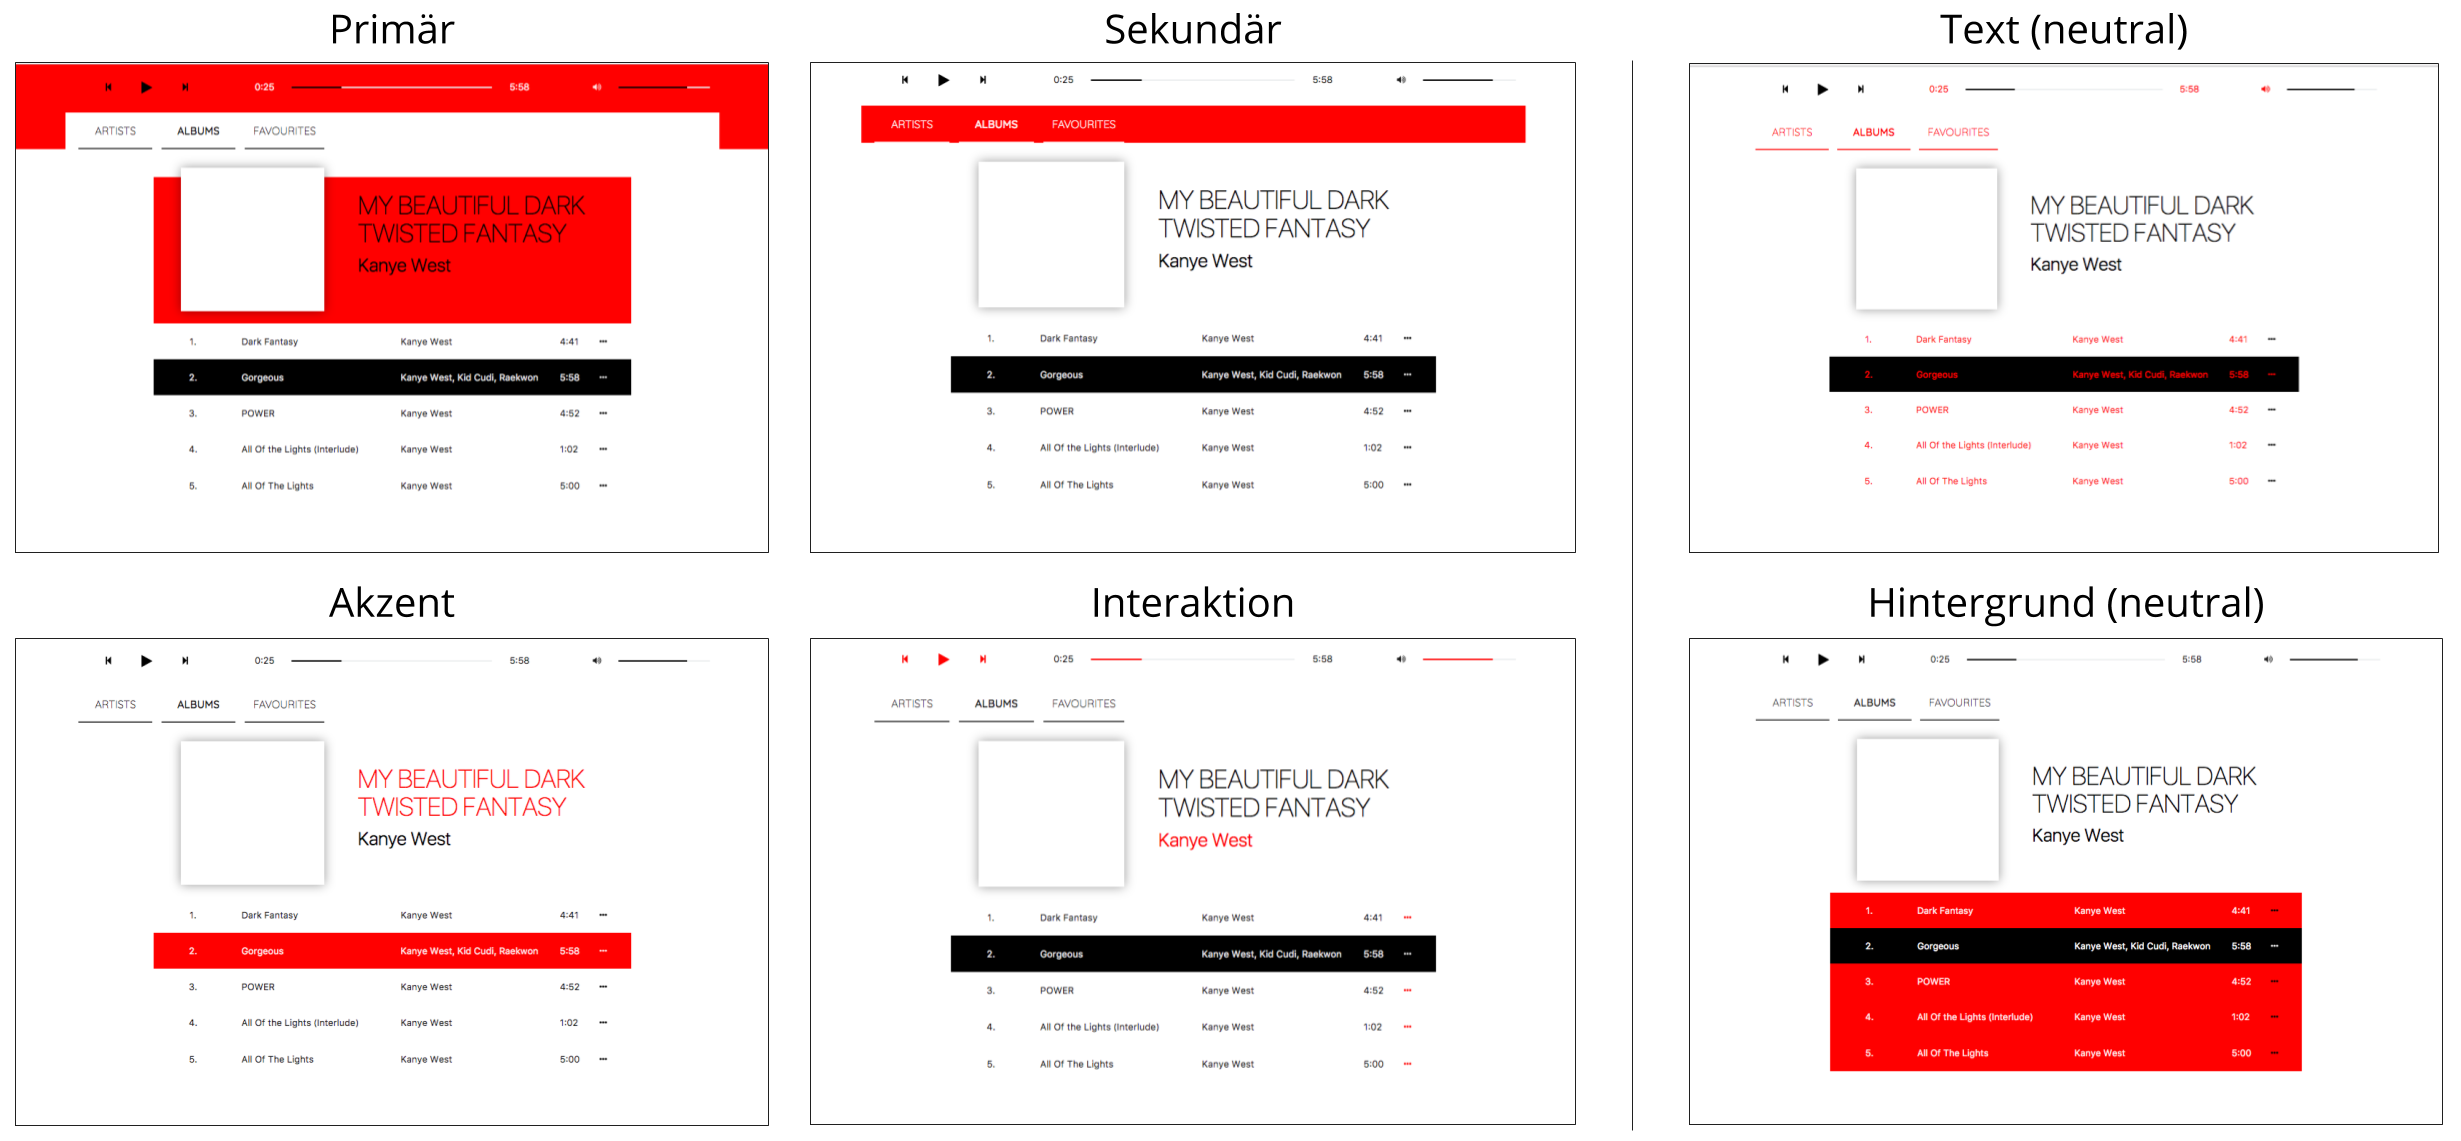
\includegraphics[width=0.95\textwidth]{img/fgs.png}
\caption{Funktionsgruppen des Layouts einer prototypischen Webseite für Musikstreaming. Alle Oberflächenkomponenten, die zur der jeweiligen Funktionsgruppe gehören, sind rot hervorgehoben.}
\label{fig:fgs}
\end{figure}

Für das Suchverfahren wurden Factor Graphs modelliert. Diese Methode wurde bereits erfolgreich in der Arbeit von \citet{magazines} zur Ermittlung der Farben von Flächen in Muster eingesetzt. Ein Factor Graph ermöglicht die Beschreibung eines Constraint Graphen. Dieser repräsentiert die Aufspaltung einer komplexen Wahrscheinlichkeitsverteilung über mehrere Variablen durch deren Zerlegung in Teilfunktionen auf einer Teilmenge der Variablen. Zur Implementierung des Graphen sowie zur Inferenz möglicher Lösungen wird die Bibliothek \emph{Dimple}\footnote{\url{http://dimple.probprog.org/}} in der Programmiersprache Java verwendet.

Der Constraint-Graph besteht aus Knoten $V$ und Kanten $E$. Knoten beschreiben Variablen, für die Werte bestimmt werden sollen. In diesem Falle gilt $V = FGs\; \backslash$ \{Text (neutral)\}. Die Gruppe \{Text (neutral)\} wird ausgelassen, da entsprechend der Erläuterungen in \autoref{sec:architektur} die Entscheidung über die Textfarbe der Blockelemente auf Layout-Ebene  getroffen wird und nicht Teil des Suchverfahrens ist. Der Wertebereich der Variablen ist eine finite Domain $dom = \{d_0, ..., d_{n+2}\}$, welche auf $P_\text{neutral} = f_{CPE}(I) \cup \{weiss, schwarz\}$ basiert, wobei die Farbwerte um weitere Attribute erweitert werden. Die Attribute der $d \in dom$ lauten:

\begin{itemize}
	\item \textbf{(H, S, I):} Der Farbwert im HSI-Raum.
	\item \textbf{Gewicht:} Akkumuliertes Gewicht aller Samples des zugehörigen Segments in der hierarchischen Farbpalette (entsprechend \autoref{eq:weight}).
	\item \textbf{Hue-Group:} Index der Hue-Group der Farbe.
	\item \textbf{Normalisierte relative Luminanz:} Berechnung entsprechend \citet{wcag-rel-luminance}.
\end{itemize}

Die Kanten entsprechen Constraints zwischen den Knoten. Es wird in Hard- und Soft-Constraints unterschieden \citep{patterns}. Hard-Constraints beschreiben Einschränkungen, die bei der Lösung des Systems nicht verletzt werden dürfen. Soft-Constraints beschreiben eine Gewichtung der möglichen Werte einer Variable in Form einer Bewertungsfunktion. So sind Eigenschaften einer Farbe beschreibbar, die sie für eine Funktionsgruppe besonders qualifizieren (z.B. eine möglichst hohe Sättigung für die Interaktionsgruppe).

In \autoref{sec:farbschemata} wurde der Typ eines Farbschemas daran unterschieden, wie viele verschiedene Farbtöne es enthält. Ein monochromes Farbschema enthält einen Farbton, ein duales zwei und ein triadisches Farbschema drei verschiedene Farbtöne. Der ACoPa-Algorithmus ermittelt die Anzahl verschiedener Farbtöne eines Bildes, wodurch ebenfalls der Typ einer Farbpalette durch Analyse der Anzahl enthaltener Hue-Groups $\#HGs(P)$ feststellbar ist. Dementsprechend führt eine Farbpalette mit $\#HGs(P) = 1$ zu einem monochromen Farbschema, eine Farbpalette mit $\#HGs(P) = 2$ zu einem dualen und mit $\#HGs(P) \geq 3$ zu einem triadischen Farbschema. Auf diese Art und Weise spiegelt sich die wahrgenommene \glqq{}Buntheit\grqq{} einer Bildvorlage (immer Sinne der Anzahl enthaltener Farbtöne) in einer entsprechend bunten Weboberfläche wieder, und umgekehrt. Farbpaletten mit mehr als drei verschiedenen Farbtönen werden auf ein triadisches Farbschema reduziert, da entsprechend \autoref{sec:farbschemata} die Verwendung von mehr Farbtönen nicht sinnvoll für die Benutzerführung ist.

Im Folgenden wird für jeden Typ ein separater Factor Graph entworfen. Die Ergebnisse werden anhand des prototypischen Layouts aus \autoref{fig:fgs} veranschaulicht.

\subsection{Triadisches Farbschema}



